\documentclass[a4paper,11pt]{article}
% \usepackage{fullpage}
% \usepackage[top=2cm, bottom=2cm, left=2cm, right=2cm]{geometry}
\usepackage[margin=2cm]{geometry}
\usepackage[charter]{mathdesign}
\usepackage{epsfig}
\usepackage{graphicx}
% \usepackage{amssymb}
% \usepackage{amsmath}
\usepackage{verbatim}
\usepackage{fancyhdr}
\usepackage{pifont}% http://ctan.org/pkg/pifont
\usepackage[rgb]{xcolor}
\usepackage{tikz}
\usetikzlibrary{matrix,positioning,fit,shapes,arrows,shadows,calc,backgrounds}
\usepackage{pgfplots}
\usepackage{natbib}
\usepackage{enumitem}
\usepackage{pgfgantt}
\usepackage{booktabs}
\usepackage{url}
\usepackage{xspace}
\usepackage{wrapfig}
\usepackage[show]{chato-notes}
\usepackage{multirow}
\usepackage[official]{eurosym}
\usepackage[bottom]{footmisc}

\usepackage{lipsum}% http://ctan.org/pkg/{graphicx,lipsum}
\newcommand{\PRLsep}{\noindent\makebox[\linewidth]{\resizebox{0.3333\linewidth}{1pt}{$\bullet$}}\bigskip}

\definecolor{verylightmagenta}{rgb}{0.95,0.96,1.0}
\definecolor{brightred}{rgb}{0.90,0.2,0.2}

\newcommand{\ag}[1]{\noindent{\color{olive}{\textbf{AG:} #1}}}
% \newcommand{\ag}[1]{}
\newcommand{\instructions}[1]{\noindent{\color{blue}{#1}}}
% \newcommand{\instructions}[1]{}

\newcommand{\mpara}[1]{\medskip\noindent{\bf #1}}
\newcommand{\spara}[1]{\smallskip\noindent{\bf #1}}
\newcommand{\para}[1]{\noindent{\bf #1}}

\newcommand{\acronym}{{\sf\small E\ensuremath{x}CLUS}\xspace}
\newcommand{\acronymtitle}{{\sf\large E\ensuremath{x}CLUS}\xspace}

\newcommand{\rto}{{RT1}\xspace}
\newcommand{\rtw}{{RT2}\xspace}
\newcommand{\rth}{{RT3}\xspace}


\newcommand{\newmodels}{{Novel explainable models}}
\newcommand{\clusterings}{{Beyond centroid-based clustering}}
\newcommand{\covariates}{{Covariate explanations}}

\newcommand{\posthoc}{{\sc PostHoc}}
\newcommand{\joint}{{\sc Joint}}


\newcommand{\proposaltitle}{{Advances in explainable clustering}}
\newcommand{\proposalabstitle}{{Advances in explainable clustering}}

\newcommand{\NP}{{\ensuremath{\mathbf{NP}}}}


%% squishlist
\newcommand{\squishlist}{\begin{list}{$\bullet$}
  { \setlength{\itemsep}{-1pt}
     \setlength{\parsep}{2pt}
     \setlength{\topsep}{2pt}
     \setlength{\partopsep}{0pt}
     \setlength{\leftmargin}{1.5em}
     \setlength{\labelwidth}{1em}
     \setlength{\labelsep}{0.5em} } }
\newcommand{\squishend}{
\end{list}  }


%% gantt stuff

% \definecolor{foobarblue}{RGB}{0,153,255}
% \definecolor{foobaryellow}{RGB}{234,187,0}
% \newganttchartelement{foobar}{
%     foobar/.style={
%         shape=rounded rectangle,
%         inner sep=0pt,
%         draw=foobarblue!50!black,
%         very thick,
%         top color=white,
%         bottom color=foobarblue!50
%     },
%     foobar incomplete/.style={
%         /pgfgantt/foobar,
%         draw=foobaryellow,
%         bottom color=foobaryellow!50
%     },
%     foobar label font=\slshape,
%     foobar left shift=-.1,
%     foobar right shift=.1
% }

%% tikz stuff

\pgfdeclarelayer{background}
\pgfdeclarelayer{foreground}
\pgfsetlayers{background,main,foreground}


\makeatletter
\tikzset{multicircle/.style  args={#1, #2}{%
 alias=tmp@name, % 
  postaction={%
    insert path={
     \pgfextra{% 
     \pgfpointdiff{\pgfpointanchor{\pgf@node@name}{center}}%
                  {\pgfpointanchor{\pgf@node@name}{east}}%            
     \pgfmathsetmacro\insiderad{\pgf@x}%
     %\foreach \c [count=\ci from = 0, evaluate=\ci as \angle using 360 - (\ci) * #1] in {#2}%
        \fill[white] (\pgf@node@name.center)  circle (\insiderad-\pgflinewidth);%
        \draw[#2] (\pgf@node@name.center)  circle (\insiderad-\pgflinewidth);%
        \fill[#2] (\pgf@node@name.center)  -- ++(0:\insiderad-\pgflinewidth) arc (0:#1:\insiderad-\pgflinewidth)--cycle;%
        }}}}}
\makeatother

\definecolor{yafaxiscolor}{rgb}{0.3, 0.3, 0.3}
\definecolor{yafcolor1}{rgb}{0.4, 0.165, 0.553}
\definecolor{yafcolor2}{rgb}{0.949, 0.482, 0.216}
\definecolor{yafcolor3}{rgb}{0.47, 0.549, 0.306}
\definecolor{yafcolor4}{rgb}{0.925, 0.165, 0.224}
\definecolor{yafcolor5}{rgb}{0.141, 0.345, 0.643}
\definecolor{yafcolor6}{rgb}{0.965, 0.933, 0.267}
\definecolor{yafcolor7}{rgb}{0.627, 0.118, 0.165}
\definecolor{yafcolor8}{rgb}{0.878, 0.475, 0.686}
\definecolor{yafcolor9}{rgb}{0.965, 0.733, 0.767}

\newlength{\yafaxispad}
\setlength{\yafaxispad}{-4pt}
\newlength{\yaftlpad}
\setlength{\yaftlpad}{\yafaxispad}
\addtolength{\yaftlpad}{-0pt}
\newlength{\yaflabelpad}
\setlength{\yaflabelpad}{-2pt}
\newlength{\yafaxiswidth}
\setlength{\yafaxiswidth}{1.2pt}
\newlength{\yafticklen}
\setlength{\yafticklen}{2pt}

\makeatletter
\def\pgfplots@drawtickgridlines@INSTALLCLIP@onorientedsurf#1{}
\makeatother

\newcommand{\yafdrawxaxis}[2]{
	\pgfplotstransformcoordinatex{#1}\let\xmincoord=\pgfmathresult 
	\pgfplotstransformcoordinatex{#2}\let\xmaxcoord=\pgfmathresult 
	\pgfsetlinewidth{\yafaxiswidth} 
	\pgfsetcolor{yafaxiscolor}
	\pgfpathmoveto{\pgfpointadd{\pgfpointadd{\pgfplotspointrelaxisxy{0}{0}}{\pgfqpointxy{\xmincoord}{0}}}{\pgfqpoint{-0.5\yafaxiswidth}{\yafaxispad}}}
	\pgfpathlineto{\pgfpointadd{\pgfpointadd{\pgfplotspointrelaxisxy{0}{0}}{\pgfqpointxy{\xmaxcoord}{0}}}{\pgfqpoint{0.5\yafaxiswidth}{\yafaxispad}}}
	\pgfusepath{stroke}

}
\newcommand{\yafdrawyaxis}[2]{
	\pgfplotstransformcoordinatey{#1}\let\ymincoord=\pgfmathresult 
	\pgfplotstransformcoordinatey{#2}\let\ymaxcoord=\pgfmathresult 
	\pgfsetlinewidth{\yafaxiswidth} 
	\pgfsetcolor{yafaxiscolor}
	\pgfpathmoveto{\pgfpointadd{\pgfpointadd{\pgfplotspointrelaxisxy{0}{0}}{\pgfqpointxy{0}{\ymincoord}}}{\pgfqpoint{\yafaxispad}{-0.5\yafaxiswidth}}}
	\pgfpathlineto{\pgfpointadd{\pgfpointadd{\pgfplotspointrelaxisxy{0}{0}}{\pgfqpointxy{0}{\ymaxcoord}}}{\pgfqpoint{\yafaxispad}{0.5\yafaxiswidth}}}
	\pgfusepath{stroke}
}

\newcommand{\yafdrawaxis}[4]{\yafdrawxaxis{#1}{#2}\yafdrawyaxis{#3}{#4}}

\pgfplotscreateplotcyclelist{yaf}{% 
{yafcolor1,mark options={scale=0.75},mark=o}, 
{yafcolor2,mark options={scale=0.75},mark=square},
{yafcolor3,mark options={scale=0.75},mark=triangle},
{yafcolor4,mark options={scale=0.75},mark=o},
{yafcolor5,mark options={scale=0.75},mark=o},
{yafcolor6,mark options={scale=0.75},mark=o},
{yafcolor7,mark options={scale=0.75},mark=o},
{yafcolor8,mark options={scale=0.75},mark=o}} 

\pgfplotsset{axis y line=left, axis x line=bottom,
	tick align=outside,
	compat = 1.3,
	tickwidth=\yafticklen,
	clip = false,
	every axis title shift = 0pt,
    x axis line style= {-, line width = 0pt, opacity = 0},
    y axis line style= {-, line width = 0pt, opacity = 0},
    x tick style= {line width = \yafaxiswidth, color=yafaxiscolor, yshift = \yafaxispad},
    y tick style= {line width = \yafaxiswidth, color=yafaxiscolor, xshift = \yafaxispad},
    x tick label style = {font=\scriptsize, yshift = \yaftlpad},
    y tick label style = {font=\scriptsize, xshift = \yaftlpad},
    every axis y label/.style = {at = {(ticklabel cs:0.5)}, rotate=90, anchor=center, font=\scriptsize, yshift = -\yaflabelpad},
    every axis x label/.style = {at = {(ticklabel cs:0.5)}, anchor=center, font=\scriptsize, yshift = \yaflabelpad},
    x tick label style = {font=\scriptsize, yshift = 1pt},
    grid = major,
    major grid style  = {dash pattern = on 1pt off 3 pt},
	every axis plot post/.append style= {line width=\yafaxiswidth} ,
	legend cell align = left,
	legend style = {inner sep = 1pt, cells = {font=\scriptsize}},
	legend image code/.code={%
		\draw[mark repeat=2,mark phase=2,#1] 
		plot coordinates { (0cm,0cm) (0.15cm,0cm) (0.3cm,0cm) };% 
	} 
}



% \setcounter{page}{1}

\renewcommand{\baselinestretch}{1.00} 
\begin{document}


\begin{center} 
% {\large Vetenskapsrådet: Distinguished professor grant within natural and engineering sciences 2024} \vspace{2.5mm}\\
{\Large Research plan} \vspace{3mm}\\
{\Large\bf {\proposaltitle} {\sc (}{\acronymtitle}{\sc )}}  \vspace{3mm} \\
{\Large Aristides Gionis} 
\end{center}

% \instructions{
% The research plan shall be forward-looking and consist of a brief but complete description of the research task. It may cover a maximum of 10 page-numbered A4 pages in Arial, font size 11, single line spacing and 2.5 cm margins, including references and any images. The research plan must include the following headings and information, listed in the following order:
% }

\subsection*{1~~~Purpose and aims}

% \instructions{
% State the overall purpose and specific aims of the research project.
% }

The explosive growth of artificial intelligence (AI) research and wide adoption of machine learning (ML) methods 
has revolutionized numerous facets of modern knowledge society, 
playing pivotal roles in decision-making, predictive analytics, optimization tasks, and beyond. 
However, a crucial issue lies in the opacity of many existing algorithms, 
hindering understanding and accountability of machine-learning methods. 
As these methods increasingly influence critical decisions in areas such as 
healthcare, finance, and criminal justice, 
there is a growing recognition of the need for \emph{transparency}, 
\emph{interpretability}, and \emph{explainability}.
Stakeholders rightfully demand explanations for algorithmic decisions, 
as well as insights into the factors driving those decisions. 
In response to the imperative for \emph{responsible AI} and the fundamental \emph{right to explanation}, 
there has been a rising focus on developing transparent and interpretable models.

Research efforts aimed at enhancing the explainability and interpretability 
of machine-learning models and methods focus on several key directions. 
First, there is a significant emphasis on developing transparent and interpretable 
\emph{white-box models}~\cite{loyola2019black}, 
such as decision trees, rule-based systems, and linear models, 
which inherently provide insights into their decision-making processes. 
Second, a significant body of research focuses on exploring \emph{post-hoc explanation techniques}, 
including feature importance analysis~\cite{lundberg2017unified} and 
model-agnostic methods~\cite{ribeiro2016model}, 
which aim to explain predictions of complex \emph{black-box models}, 
such as deep neural networks or ensemble methods.

% chatGPT text below
% Additionally, there is a growing interest in integrating domain knowledge and human feedback into the model training process, facilitating the creation of more interpretable and trustworthy models.  Moreover, efforts are directed towards developing evaluation metrics and benchmarks  to assess the quality and reliability of explanations provided by these methods.  Finally, interdisciplinary collaboration between researchers in machine learning, cognitive science, and ethics is crucial for addressing societal concerns and ensuring the responsible deployment of explainable AI systems.

Much of research discussed in the previous paragraph focuses on \emph{supervised machine-learning methods}, 
e.g., classification, object recognition, and natural-language processing, among other.
On the other hand, significantly less attention has been given on the 
topic of explainability and interpretability for \emph{unsupervised machine learning}.
The most typical tasks in unsupervised machine learning include
\emph{data clustering}, \emph{outlier detection}, \emph{network analysis}, and more. 
In this project we will focus on the problem of \emph{explainable clustering}, 
although some of our ideas can be also extended to other tasks.

Clustering is a fundamental task in data analysis and machine learning, 
seeking to partition data into groups based on their similarity.
Clustering algorithms enable data scientists and practitioners
to uncover hidden patterns, extract meaningful insights, 
and make informed decisions without the need for labeled data. 
Clustering plays a pivotal role in various domains
% , including  document analysis, bioinformatics, and recommendation systems, 
while it also serves as a preprocessing step for other machine-learning tasks, 
helping to streamline feature engineering, visualization, and model~building.

Although hugely popular, 
traditional clustering methods often lack transparency in explaining 
why certain data points are grouped together, 
thus necessitating a manual validation process to make sense of the clustering. 
As the data complexity keeps growing, 
it becomes increasingly hard to understand the reasons behind a clustering.
While many clustering methods rely on optimizing simple-to-state objective functions, 
the resulting clusterings are not always simple to explain. 
Furthermore, numerous clustering methods use opaque approaches
for which explanations are not available. 
Examples include density-based approaches, spectral techniques, embedding methods,  
agglomerative strategies, self-organizing maps, and~more.

Recognizing the need for transparent and explainable clustering methods, 
researchers have recently proposed ideas and techniques for finding 
interpretable reasoning behind clusters.
While a review of those methods is presented in the next section, 
most notable examples include 
explaining a black-box clustering using decision trees~\cite{gupta2023price,moshkovitz2020explainable},
descriptive labels~\cite{davidson2018cluster,sambaturu2020efficient}, 
\textcolor{red}{or \ldots}.

\spara{Challenges and limitations.}
While these methods present many novel ideas and make significant advances, 
many challenges remain and there is ample space for fruitful research in this important topic. 
In particular, existing methods fail to integrate with the most common variants of kernel-based clustering, 
thus failing to yield explainable clusters on models exploiting non-linear similarities.
Second, existing methods do not cater to real-world data challenges where data has special features, 
labels, or covariates, as they cannot distinguish between special covariate features and data features.
Additionally, out of the large toolbox of explainable machine-learning models,
decision trees have primarily been used for explanations, 
while other models could be better suited for certain applications. 
Last but not least, while the majority of existing methods focus on explaining black-box clusterings, 
it is often important to \emph{a priori} cluster the data so that the result complies 
by-design with a family of explainable models.
Our objective in this project is to address many of these challenges
and make significance advances in the topic of explainable clustering.

\medskip
\noindent
\hspace{-3mm}\colorbox{verylightmagenta}{
\begin{minipage}{\textwidth}
{\bf High-level goal of \acronym:} 
We will develop novel theoretical frameworks for 
introducing transparency and explainability into the task of data clustering. 
We will develop explainable clustering methods that employ novel white-box models, 
and we will devise methods for providing explanations to clusterings produced by complex clustering models.
Furthermore, we will study formulations that leverage special features of the data,
such as labels and covariates.
\end{minipage}}

\mpara{Research objectives.}
To achieve our objective of advancing the state of the art in explainable clustering
we aim to consolidate existing approaches,  including our own work,  
introduce novel abstractions, 
develop rigorous computational methods, and 
perform evaluations on real-world datasets.
In particular, {\acronym} has the following research objectives. 

\vspace{-2mm}
\begin{description}
\setlength{\itemsep}{-4pt}
\item[{Models and problems:}]
Develop novel models and novel problem formulations that enable 
obtaining a deeper understanding of the problem of explainable clustering.
Focus on three themes: 
\emph{novel explainable models}, 
\emph{explainability beyond centroid-based clustering}, and 
\emph{explaining clustering with covariates}.

\item[{Algorithms:}]
Develop computational methods for the problems that will be formulated.
Our methods will rely on different techniques
including combinatorial optimization, approximation algorithms, and linear algebra.
The proposed algorithms should be efficient and should offer theoretical guarantees.

\item[{Empirical evaluation and outreach:}]
Implement the proposed methods and evaluate them on 
real-world benchmark datasets from different application areas.
Collaborate with experts in other areas for applying the methods in their domain.
% Validate proof-of-concept by showcasing findings of the methods on different use cases. 
Make the implementation of our methods available to the scientific community.

\item[{Education in KTH:}]
Support a new doctoral student in KTH, 
educate them on algorithmic data analysis and responsible AI. 
Create an environment of collaboration for the new doctoral student 
with postdocs in the group of the PI, working on the same topic, 
as well as with other researchers in the international collaboration network of the PI.
\end{description}

\vspace{-2mm}
\noindent
We next discuss briefly the state of the art
before presenting the proposed approach.

\subsection*{2~~~State of the art}

% \instructions{
% Summarize briefly the current research frontier within the field or area covered by the project. State key references.
% }

Algorithmically grouping similar data points has a long research history,
yielding traditional methods, 
such as $k$-means~\cite{macqueen1967some}, 
DBSCAN~\cite{ester1996ada}, or spectral clustering~\cite{ng2001spectral}.
Methods to enhance cluster interpretability have long been focused on subspace clustering~\cite{rubinstein2010dict}, 
% (such as $k$-SVD~\cite{rubinstein2010dict}), 
feature importance measures, such as Shapley values \cite{lundberg2017unified}, 
or dimensionality-reduction techniques~\cite{hinton2002tsne,lee2000algorithms,mcinnes2018umap}.
% (such as $t$-SNE~\cite{hinton2002tsne}, UMAP~\cite{mcinnes2018umap}, or NMF~\cite{lee2000algorithms}).
From the sprawling explainable machine-learning research, the area of explainable or interpretable clustering has emerged, aiming to rationalize the underlying reasons for clusters. 
Our proposed research may be seen as being situated in this dynamic and active research area, whose state-of-the-art we will sketch in the following. 

Considerable attention has been given to \emph{explaining clusters} with decision trees, 
including explaining using similarity-based prototypes for each cluster \cite{carrizosa2022interpreting}, 
or by fitting oblique trees to describe clusters \cite{gabidolla2022optimal}.
In the seminal work, Moshkovitz et al.~\cite{moshkovitz2020explainable} 
explain $k$-means and $k$-medians with axis-aligned decision trees, 
deriving a worst-case approximation guarantee, termed as ``price of explainability,'' 
inspired by the ``price of interpretability'' \cite{bertsimas2019price} for axis-aligned decision tree classification. 
Recent developments focus on improving worst-case bounds on explainability for $k$-means, 
by using random threshold cuts for axis-aligned decisions 
\cite{makarychev2022explainable, esfandiari2022almost, makarychev2023random}. 
The best known upper bound on the price of explainability for $k$-means is 
$\mathcal{O}(k \log \log k)$ \cite{gupta2023price}, 
with a known lower bound of $\Omega(k)$ \cite{gamlath2021explainable}.

As narrow the gap already is, 
it can further be improved for low-dimensional problems \cite{charikar2022near,laber2021price}. 
Aiming for a slight generalization, the restriction that decision trees have to have $k$ leaves has been removed, improving the worst-case guarantees \cite{makarychev2022explainable} and 
showing good performance in practice \cite{frost2020exkmc}. 
Now free of this restriction trees can grow larger.
As such growth inhibits interpretability, 
Laber et al.~\cite{laber2023nearly} explore shallow decision trees for explainable clustering, 
while Deng et al.~\cite{deng2023impossibility} demonstrate 
that shallow trees for explainable $k$-means and $k$-medians is impossible to achieve in general. 
Further research includes explainability for $k$-centers~\cite{laber2021price} or 
explainable clustering under $\|\cdot\|_p$-norms \cite{gamlath2021explainable}. 
Research on explaining kernel $k$-means has only recently been started, 
showing that axis-aligned trees lead to approximation guarantees for a limited set of interpretable kernels, 
while showing an \emph{unbounded} ``price of explainability'' 
for explaining the widely-used quadratic kernel \cite{fleissner2024explaining}.

In summary, recent advances focus on explaining (mostly) $k$-means clusters with (mostly) axis-aligned trees. 
Research on more expressive explanation like oblique decision trees or complex clustering 
like kernel $k$-means is still in its infancy.

Closely related to our proposal is research in the area of \emph{interpretable clustering},
seeking to compute inherently interpretable clusters \emph{without} resorting to post-hoc explanations.
Recent research has focused on aiding clustering towards interpretable solutions by directly integrating 
decision-tree explanations into the clustering algorithm,
One approach leverages \emph{mixed integer linear programming} 
to derive an interpretable tree-based clustering algorithm 
by approximating the globally-optimal solution~\cite{bertsimas2021interpretable}. 
Also building on combinatorial optimization, a different approach increases the expressivity 
while decreasing interpretability, 
by leveraging soft decision trees~\cite{cohen2023interpretable} as a guide for $k$-means. 
A different take on explainability or interpretability for clusterings 
moves away from explaining centroids or data points 
but describes clusters boundaries with polyhedra, 
again using combinatorial optimization~\cite{lawless2023polyhedral}. 

% Some clustering algorithms aim to find interpretability fro embeddings via \textbf{dimensionality reduction} algorithms such as nonnegative matrix factorization \cite{} or tensor decompositions \cite{}.    
% Related to our research themes are inherently \textbf{interpretable machine learning} methods,
% employable as substitutes for the decision tree models, for example 

% Classic approaches that are related to explainable clustering include \textbf{subspace clustering} which aims at discovering clusters in high-dimensional data by assuming that data points only belong to certain lower-dimensional subspace clusters rather than being globally clustered, thus enhancing interpretability.
% While many subspace methods such as $k$-SVD~\cite{} focus on subspace selection, explanations emphasizes understanding the rationale behind clusters, which often in practice is elucidated with feature importance analysis.
% While selecting the top most important features for clustering  
% An important research area lies in measuring and ranking \textbf{feature importance} for clusters.   
% In the context of explainable clustering, measuring the feature importance falls into two categories:
% \emph{unsupervised} if no clusters are given (\joint) and \emph{supervised} if clusters are given (\posthoc).


\subsection*{3~~~Significance and scientific novelty}

% \instructions{
% Describe briefly how the project relates to previous research within the area, and the impact the project may have in the short and long term. Describe also how the project moves forward or innovates the current research frontier.
% }

\para{Significance.} Our project lies in the intersection of the areas of  
algorithms design, knowledge discovery, and explainable machine learning.
The problem domain we propose to study, 
explainability in unsupervised machine learning and data clustering, 
will enable scientists and practitioners in  different application areas to 
make better sense of their data. 
It will do so by not only allowing them to find meaningful clusters
but also by helping the to understand the fundamental mechanisms in the creation of clusters, 
the importance and contribution of features, and ways to explain the clusters
with covariate attributes.

\spara{Scientific novelty.} 
The project will make contributions in several different directions. 
The area of trustworthy, transparent, and explainable machine learning 
has gained a lot of traction in recent years, but most of the attention
has been given in the area of supervised machine learning. 
The topic of explainability in unsupervised machine learning, 
and in particular in data clustering, 
is not completely unexplored, 
but overall, the area is mostly at its infancy and 
most of the works fall within a few frameworks. 
Here we propose to significantly enlarge the scope of research in this particular domain, 
and we propose many novel directions, 
such as using other interpretable machine-learning models to explain a given clustering result, 
providing explainability for complex, beyond centroid-based clustering, 
and finding optimal clusterings in conjunction with short explanations using covariate attributes. 
Our work will be foundational in nature, 
focusing on methods that provide formal guarantees, 
and leveraging ideas from combinatorial optimization, 
information theory, probabilistic algorithms, and statistical learning theory.

\subsection*{4~~~Preliminary and previous results}

% \instructions{
% Describe briefly your own previous research and pilot studies within the research area that make it probable that the project will be feasible. If no preliminary results exist, please state this too. State also whether the project contributes further to research and scientific results from a grant awarded previously by the Swedish Research Council.
% }

The PI is in a unique position to accomplish the goals of the project. 
His profile brings together theoretical work on algorithmic data analysis, 
with development of practical data-mining methods, and emphasis on applications. 
While the PI has not worked directly on the problem of explainable clustering,
he has published numerous high-impact articles on other related computational tasks, 
including work on data clustering and explainable machine learning. 

With respect to clustering, 
the earlier work of the PI includes papers on
\emph{correlation clustering}~\cite{bonchi2013overlapping,gionis2007clustering},
unified framework for \emph{clustering with outlier detection}~\cite{chawla2013k},
\emph{kernelized clustering}~\cite{amid2015kernel}, and more.
Most recent work includes papers on
\emph{diversity-aware clustering}~\cite{thejaswi2021diversity}, 
which is a formulation asking for cluster centers being diverse with respect to covariate attributes, and
\emph{reconciliation clustering}~\cite{spoerhase2023constant}, 
which is a formulation asking to avoid selecting cluster centers that are far away to each other.
None of these problems provides an explainable clustering, 
thus, it would be interesting to study whether we can introduce explainability
into these formulations.
%
With respect to explainable machine learning, 
the PI has published papers on 
\emph{explainable time-series classification with counterfactual analysis}~\cite{karlsson2020locally},
\emph{explainable rule-based classification models}~\cite{ciaperoni2023concise,zhang2020diverse}
and 
\emph{explainable decision-tree models}~\cite{zhang2023regularized}. 
Related to this project is also the work
finding dense subgraphs with covariate explanations~\cite{galbrun2014overlapping,galbrun2016top}.
We believe that ideas and techniques from that line of work
will be very relevant to the third research theme of this project.

A member of the research team of the PI is postdoctoral researcher Sebastian Dalleiger, 
who will contribute to this project by supervising the recruited PhD student.
Dr.\ Dalleiger has expertise on many aspects of theoretical machine learning, 
including highly relevant work on \emph{explainable data decompositions}~\cite{dalleiger2020explainable}
statistically \emph{significant feature interactions}~\cite{dalleiger2022spass}, 
or \emph{matrix factorization}~\cite{dalleiger2022efficiently}.

\subsection*{5~~~Project description}

%\instructions{
%Describe the project design under the following headings:
%}

\subsection*{5.1~~~Theory and methods}

%\instructions{
%Describe the underlying theory and the methods to be applied in order to reach the project goal.
%}

The project is structured along three {\em research themes}:

\vspace{-2mm}
\begin{description}
\setlength{\itemsep}{-2pt}
\item[\rto.~\newmodels\,:] 
Explain clustering using a richer family of interpretable machine-learning models, 
including oblique decision trees, Bayesian decision rules, cascading rule lists, and 
generalized linear models. 
Develop methods to finding interpretable cluster explanations 
via highlighting the importance of features and the feature interactions for each cluster.

\item[\rtw.~\clusterings\,:] 
Develop methods to explain more complex clustering structure than centroid-based methods,
for example, clustering that have resulted by kernel $k$-means or density-based formulations.

\item[\rth.~\covariates\,:]
Develop methods for obtaining high-quality clusterings of data 
while using the covariate attributes for explaining the resulting clusterings. 
In this theme we aim to minimize clustering cost, based on vector-based representations, 
while achieving high expressivity and high specificity of the clusterings, 
based on covariate attributes.

\end{description}

\vspace{-2mm}
When considering different approaches for explainable clustering we distinguish between 
two different computational paradigms. 

% \vspace{-2mm}
% \begin{description}
% \setlength{\itemsep}{-2pt}

\smallskip
% \noindent
{\posthoc\,:}
In the first paradigm, we assume that a clustering of the data is provided 
by a \emph{black-box clustering method} and the problem objective is to design 
a \emph{post-hoc} explanation of the input clustering.
This task is similar to \emph{explainable machine learning}, 
where one asks to develop post-hoc interpretable justifications for 
\emph{black-box classification models}, such as neural networks. 

\smallskip
% \noindent
{\joint\,:}
In the second paradigm the goal is to find an optimal clustering of the data
from a family of explainable clustering models.
That is, one needs to \emph{cluster the data} and \emph{select the explainable clustering model}
in a \emph{joint manner}.
In the general case, the clustering cost incurred by an inherently interpretable model 
will be larger than the cost incurred by an optimal (but non-explainable) model, 
so our goal will be to bound the cost of the interpretable model with respect to the optimal cost.
% \end{description}

\smallskip
Next we discuss in more detail the three research themes of \acronym.
We present formulations both in \posthoc\ and \joint paradigms.

% The two paradigms, \posthoc\ and \joint, are present in all three of our research themes.
% When discussing different explainable-clustering approaches 
% we specify the paradigm for a specific approach.

\subsection*{Research theme 1 (\rto): \newmodels}

At the core of many data-analysis questions lies the task of discovering clusters in data. 
In many cases we are interested not only in what are the prominent clusters, 
but also which mechanisms are responsible for them,  
what are their characteristics, and how to tell them apart.  
A medical scientist, for example, may want to determine the factors that tell apart 
high-risk from low-risk clusters, 
or may seek to highlight the characteristics that are specific to a disease cluster.  
% How can we explain clusters with sets of specific features with particularly observed values?

A broadly-used \posthoc approach in explaining \emph{pre-existing} $k$-means clusters uses 
\emph{axis-aligned decision trees}. 
That is, to attribute data to clusters, 
we only have to mechanistically answer a sequence of yes-no questions, 
which have been algorithmically derived from data features, 
thereby describing clusters with easily understandable and inherently interpretable axis-aligned rules (cuts), 
such as 
``\texttt{if} $x_i \in [\textnormal{lb}, \textnormal{ub}]$ \texttt{then} 
proceed with left subtree \texttt{else} proceed with right subtree \texttt{end} until a cluster at a leaf is reached.''
Reaching clusters by means of such an interpretable model incurs 
a cost in addition to the original $k$-means clustering cost, 
which is called \emph{the price of explainability}.
Central to our research is the question of how large the price to pay becomes, i.e., 
what is the worst-case achievable approximation guarantee of expressing a clustering 
in terms of a specific interpretable machine-learning model. 

Although the price for explaining $k$-means with axis-aligned decision tree might be low~\cite{gupta2023price}, 
a recent investigation~\cite{deng2023impossibility} shows that the cost lies in the size of the tree.
Simply put, a precise explanation requires large trees.
The larger the clustering complexity, the larger the explanations, thereby 
% shrinking interpretability to a point where 
the benefits of having an explanation over analyzing raw data diminishes.
The bottom line is: there is more to explainability than guaranteeing a clustering quality under interpretable rules.
A core challenge of explainable clustering is to identify how to properly quantify explainability,
what are good explanations, and how well do they address real-world circumstances in theory and practice.
We propose to holistically explore new kinds of explanations to enhance explainable clustering,
by advancing decision trees, exploring rule-based explanations, and by investigating important features for clusters.

First, we plan to explore advanced decision tree models with more expressive individual decision function per node, aiming to guarantee concise explanations even when considering complex data.
The principle is simple: the more expressive individual decision functions are, the fewer decisions we need to make. 
One avenue leads to oblique decision trees, whose decision functions generalize simple axis-aligned decision-making to hyperplane-based decision-making, akin to $\mathbf{a}_i^{\!\top} \mathbf{x}^{\vphantom{\top}}_{\vphantom{i}} + b_i$. % < 0
The danger of employing expressive decision functions, however, lies in the increased complexity of each individual decisions functions, thus negatively impacting individual interpretability.
Therefore, a core challenge of this research theme is the question of how to find expressive functions that balance individual interpretability, overall explainability, and accuracy.
In the context of hyperplanes $\mathbf{a}_i^{\!\top} \mathbf{x}^{\vphantom{\top}}_{\vphantom{i}} + b_i < c_i$, for example, we seek to reduce the complexity of individual hyperplanes using non-negativity constraints $\mathbf{a} \in \mathbb{R}^m_{\geq 0}$ and sparsity \emph{constraints} $\|\mathbf{a}\|_0 \leq q$, by employing combinatorial optimization techniques for small problems or (greedy) subspace algorithms such as orthogonal matching pursuit, sequential lasso, or top-$q$ important feature forward selection for large problems.

An alternative approach is to go beyond decision trees to explore other models capable of explaining clusters. 
Machine-learning models such as Bayesian decision rules, cascading rule lists, and generalized linear models 
are prime candidates to explore, given their widespread adoption and inherent interpretability. 
One concrete goal is to study how we can explain clusters with concise decision rule lists 
of the form ``\texttt{if} $\bigwedge_i \llbracket x_i \in [\textnormal{lb}, \textnormal{ub}] \rrbracket$ 
\texttt{then} cluster$_a$ \texttt{else} proceed with the next rule \texttt{end}.'' 
By exploiting the additional modeling flexibility, 
we specifically aim to investigate explainable clustering for \emph{knowledge-seeking applications}, 
where an under-researched problem is that (rule-based) explanations 
often repeat already-known salient signals, thus failing to convey new knowledge.
For example, 
% if the algorithm accurately explains a cluster `\texttt{\small ClimateCrisis}' in terms of a high concentration of `\texttt{\small CO\textsubscript{2}}', it would fail to tell us about `\texttt{\small methane}'; or 
an explanation of `\texttt{\small Diabetes}' with a highly-expressed 
but known-to-be-relevant gene `\texttt{\small TCF7L2}', 
might hide an almost equally relevant gene `\texttt{\small ZNT8}'.  
As the algorithm does not know in advance which explanations are most informative to the user, 
we aim to provide sets of explanations that offer \emph{diverse perspectives} on the clustering.
In the context of rule sets $\mathcal{R} = \{r_1, \dots, r_n\}$, 
we seek to explain a clustering $Y$ of data points $X$ 
by minimizing the loss $\ell(\mathcal{R},Y;X)$ between explained clustering and the estimated clustering 
penalized by the rule diversity~$d(\mathcal{R})$, 
that is, minimizing $\ell(\mathcal{R},Y;X) + \lambda \operatorname{d}(\mathcal{R})$~\cite{zhang2020diverse}.
% \ag{Do you want to include more details, e.g., about \textsc{MaxSum} diversification?}
So far, diverse explanations for clustering is an understudied subject, and quality, conciseness, and empirical performance are unknown. 
We aspire to change this by studying the theoretical underpinning, the price of diversity for explainability clustering, its practical implication on clustering accuracy, and the ability to acquire new knowledge. 

A major challenge of finding interpretable explanations is in judging the importance of data features per cluster.
Having an importance measure allows us to explain clusters in terms of importance `spectra' such as $\{\slifI,\slifII,\slifIII\}$, thereby highlighting informative feature-values that are characteristic, contrastive, or common in clusters.
% In this example, we notice that feature $1$ and $2$ are significantly more important to cluster $b$ than $a$ or $c$.
Although importance measures such as Shapely values or impurity typically consider features independently, 
in reality, features often interact with each other.
We hypothesize that features interact differently per cluster and that differences in those interactions are relevant reasons for specific clusters, as evidenced in our prior work~\cite{dalleiger2020explainable}.

We plan to investigate novel higher-order importance measures to highlight the characteristics or contrastive per-cluster feature-interactions, leveraging ideas from information theory, statistics, and statistical learning.
However, research on the importance of higher-order feature interactions for data clusters is still lacking, 
as this poses significant algorithmic and statistical challenges, by involving exponentially many potential interactions for which non-linear or multi-variate analytics is necessary to compute importance.  
We plan to explore novel measures to judge the importance of higher-order feature interactions, leveraging ideas from information theory, statistics, and statistical learning, thus highlighting sets of important feature-interactions that are relevant for clusters.

\iffalse
\note{Solution details? Should we remove this section?}

Regardless of expressivity, any \posthoc explanation has to explain \emph{pre-existing} clusters of almost arbitrary complexity.
Colloquially speaking, that is because the clustering algorithm does not know that we want explainability.
How can we make clustering aware of the explainability of its result?
An important aspect of \rto is the question of how to incorporate explanations into clustering as a \joint problem.
For classical $k$-means, for example, one obvious objective $\arg\;\min_{e, w, c} \sum_j \sum_i P_{ki}(e) w_{ki} \| x_i - c_j \|$ augments the $k$-means objective with a probability or weight $P_{ki}$ that our explanation $e$ concludes that data point $x_i$ is in cluster $j$. 
In case that $E$ is an oblique decision tree, for example, the probability $P_{ki}$ stems from a sequence of hyperplane-derived probabilities.
We hope to explore the cost that joining explanations with clustering would inflict on the clustering performance, computational complexity, and explainability of the results.
\fi 

% \note{

% Central to our research is the concept of the price of explainability, as the worst-case achievable approximation guarantee of expressing a clustering in terms of a different interpretable machine learning model.

% Given a clustering produced by any black-box clustering method, e.g., $k$-means,
% provide explanations of the clustering using models that go beyond axis-aligned decision trees.
% Such models include 
% (i) non-axis aligned decision trees;
% (ii) decision rules or decision lists;
% (iii) ??
% Here we can also include work on explaining clusterings using feature importance. 

% Existing methods that explain clustering results with axis-aligned decision trees
% provide quality guarantees.
% Ensuring that our methods, will provide quality guarantees for the novel models
% we will introduce is a major challenge for this research theme.

\subsection*{Research theme 2 (\rtw): \clusterings}

Most related recent research on explainable clustering has focused on classical $k$-means,
thereby resulting in algorithms that approximate $k$-means clusters with axis-aligned decision trees.
However, the classical $k$-means algorithm has limited applicability in practice, as it is often not flexible enough to handle complex datasets that contain complicated cluster shapes.
So far, the price of explainability in the context of other algorithms is understudied and questions such as ``how well axis-aligned decision trees could explain DBSCAN in the worst case?'' or ``how well do oblique decision trees approximate spectral clustering or hierarchical clustering results?'' remain unanswered.
Here, we go beyond classical $k$-means towards developing explaining clustering algorithms for complex clusters.

Arguably one of the most inhibiting factors is $k$-means inability to exploit non-linearities in the relationship between data, which is often addressed by kernelized $k$-means algorithms.
Explaining kernel $k$-means, however, poses significant challenges, as clusters are harder to split apart 
with simple axis-aligned decision trees. 
In fact, a very recent advancement has discovered that the worst-case price of explaining quadratic-kernel-based clusterings with axis-aligned trees is \emph{theoretically unbounded}~\cite{fleissner2024explaining}, 
i.e., explanations can be arbitrarily bad. 
This raises some of our core challenges in \rtw:
\textbf{(1)} Is there a different explainable clustering algorithm that achieves tighter bounds under kernels,
such as the quadratic kernel for example, by incorporating explanations into the algorithm?;
\textbf{(2)} What are inherently interpretable kernels for explainable clustering?;
\textbf{(3)} How would more expressive explanations improve this bound (cf., \rto)?;
\textbf{(4)} Going beyond worst-case analysis, what are the \emph{expected} or the \emph{lower bound} to the price of explainability?; and
\textbf{(5)} Can we align approximation guarantees to the geometries of explanations and clusterings?

Building on research from \rto, we seek to relate more expressive explanations to more expressive spectral or kernel clustering,
thus understanding the prize of explainability in the light of potentially slightly reduced interpretability.
For example, if a border between clusters is a sinusoidal curve, we would probably require many axis-aligned `step' functions to separate clusters. A more expressive, yet easily understandable description would be a simple function. 
However, what if the border is not smooth and not easily explainable?
In this case, humans are willing to use simpler approximations.
Similarly, we would like to explore fuzzy explanations 
that may provide imperfect description of complicated border situations.
More concretely, can we find fuzzy or Bayesian rule sets that explain clusters with high probability, 
however with simpler terms?
We seek to study if these explanations are suitable to explain soft clustering, 
like fuzzy $c$-means, and how to develop a \joint explainable fuzzy clustering algorithm, 
which at the moment is an understudied research area.
The theoretical challenge lies in exploring if and how to adapt the prize of explainability 
for imperfect and uncertain explanations. 

We also aim to explore inherently interpretable kernel feature maps, 
seeking deterministic maps that allow us to trace similarities back to the original data features. 
We plan to explore suitably transparent kernels $\langle \phi(x), \phi(y) \rangle$ that allow 
for attributing cluster-decisions to features, 
by identifying inherently-interpretable kernel feature maps $\phi(x)$. 
The traceability might necessitate the development of novel algorithms that cluster via the kernel while extracting rules by leveraging the interpretability of the kernel. 
More generally, we see a lot of potential for developing new algorithms for interpretable kernelized clustering that steer-away from
clusters that are identifiable by our kernel but are hardly explainable in terms of less-expressive human-understandable models (such as axis-aligned decision trees), thereby allowing us to balance explainability with the power of kernel clustering.
In a similar spirit, we will explore the idea of using multiple kernels 
in which clustering is performed based on one kernel (e.g., the quadratic kernel), 
while explanations come from inherently interpretable kernels.

One potential avenue towards explainable kernelized clustering involves inherently interpretable `surrogates.'
That is, can we approximate potentially hardly-interpretable projections with simpler estimations?
Inspired by interpretable machine learning, we like to explore explainable machine-learning models that 
\emph{learn to predict how distant} data points are to one another, 
leveraging research from explainable regression (e.g., via regression tree variants) and pairwise comparison problems.
In a similar vain, we are interested in approximating kernel feature maps with interpretable embeddings. 
A core challenge involves the definition, estimation, or learning of novel explainable surrogate functions, 
or maps, to achieve a distance measure allowing for complex clusters while being strictly interpretable.
% In the area of \emph{algorithms with predictions}, we then plan to derive an algorithm for explainable clustering with predicted distances, thereby building on the interpretability of the distance matrices.

Furthermore, we hypothesize that the price of explainability differs across geometries or topologies, 
such as hyperbolic versus Euclidean spaces, 
combining ideas from geometric machine learning for explainability. 
That is, we seek to explore if specifically-structured observations (e.g., tree-like data) 
that require exponentially-sized models in Euclidean space, 
can be described in polynomial number of rules in a more appropriate (e.g., hyperbolic) space.
Sometimes, we can perfectly separate clusters in the data with only a single axis-aligned decision.
For example, an apple-shaped cluster is on the left of the $y$-axis and a banana-shaped cluster is on its right. 
The $y$-axis, however, would fail do fully explain how the clusters are different.
Inspired by robust clustering and polyhedral descriptions \cite{lawless2023polyhedral},
we hope to explore more complex geometric yet interpretable descriptions of complex clusters.
% seeking to generalize polyhedral, study shape-interpretability. 
We additionally plan to investigate approximation guarantees for complex kernel clusters and seek to develop a geometric explainable clustering algorithm.

% Here we will focus on developing methods providing explanations for clusterings 
% that go beyond centroid-based approaches like $k$-means or $k$-median.
% In particular we will consider the following clustering approaches.
% \begin{itemize}
% \setlength{\itemsep}{-2pt}
% \item kernel-based clustering
% \item density-based clustering; what would be a good model for this case?
% \item subspace clustering \hfill\ag{does this make sense?}
% \item diversity-aware (or fair) clustering \hfill\ag{does this make sense?}
% \item what if want the explanation be fair, instead of the clustering?
% \item clusterings with embeddings
% \end{itemize}

% There is strong interaction between \rto and \rtw, 
% due to the fact that providing explanations for clusterings that go beyond centroid-based methods
% will require working with novel models.

\subsection*{Research theme 3 (\rth): \covariates}

In many application scenarios data can be represented in different ways: 
Most often, data can be represented in a vector space
in which appropriate distance functions, or similarity functions, are considered.
Such a vector space can be defined using directly data features, 
or it can be learned using representation-learning techniques~\cite{hamilton2017representation,wang2020survey}.
Second, data points are associated with covariates, 
which are discrete (categorical) attributes, 
representing certain aspects of the data. 
Such covariates can be labels, tags, or other related information.
Given the discrete nature of covariates it is typically not easy (or meaningful)
to define distance functions based on them, 
although sometimes coarse-grained distance functions can be specified.

For an example illustrating the setting described above, 
consider a collection of news articles. 
Each news article can be represented by a vector in a high-dimensional space, 
e.g., using bag-of-words, \tfidf-type weighting, or deep-learning embedding schemes. 
Furthermore, for each news article we can associate a small 
set of tags, or labels, summarizing the topic of the article, 
e.g., an article reporting on climate change could be labeled by
`\texttt{\small ClimateCrisis}' and `\texttt{\small ExtremeWeather}.'
We refer to these labels as covariate~attributes.

When considering the problem of clustering a dataset in which the data points are 
represented both in vector space and with covariate attributes, 
it is immediate clear how to leverage the vectorial information
using a standard clustering method, such as $k$-means or spectral clustering. 
One of the other hand, it is not obvious how to use effectively the 
covariate attributes in order to improve the clustering results. 

In this research theme we propose finding high-quality clusterings of the data
while using the covariate attributes for explaining the resulting clusterings. 
In particular, we aim to develop novel clustering methods
that achieve low-cost solutions with respect to the vector-representation of the data points, 
while at the same time achieve high expressivity and high specificity of the clusterings
using the covariate attributes. 

To be more concrete, as one possible problem formulation that we will explore, 
let us consider a set of $n$ data points $\dataset=\{\vecx_1,\ldots,\vecx_n\}$
and a set of covariate attributes {\labelset} representing labels for the data points. 
Each data point $\vecx_i$ is associated with a set of labels $\labels_i\subseteq\labelset$. 
A set of labels $\labels=\{\alabel_1,\ldots,\alabel_k\}\subseteq\labelset$, 
henceforth referred to as \emph{descriptor set}, 
\emph{induces} a subset of the data points $\dataset(\labels)\subseteq\dataset$
via a \emph{logic grammar}, such as, for example, 
$\dataset(\labels)$ consists of the data points in \dataset that 
are associated with at least $s$ labels contained in \labels.
For the set of points $\dataset(\labels)$ induced by \labels 
we can then define its \emph{clustering cost} $d(\dataset(\labels))$, 
using the geometry of the points in the set, 
e.g., the diameter of the set, or the sum of distances of all points to the median of the set.
The problem of explainable clustering with covariate attributes that we will study is the following: 
find a collection of label sets $\labels_1,\ldots,\labels_t$, 
so that the induced clusters $\dataset(\labels_1),\ldots,\dataset(\labels_t)$
cover the whole dataset \dataset, 
and some aggregate function on the cost of the clusters is minimized. 
Natural choices for the total clustering cost are
$d_{+}(\labels_1,\ldots,\labels_t) = \sum_{j} d(\dataset(\labels_j))$ and 
$d_{m}(\labels_1,\ldots,\labels_t) = \max_{j}\! \left\{ d(\dataset(\labels_j)) \right\}$, 
that is, we will aim to minimize the total cost, or worst-case cost, respectively, 
among all clusters. 

A few observations are in order for the problem that we define above.
First we note that the problem belongs in the \joint paradigm, 
that is, we aim to \emph{simultaneously} find a low-cost clustering, 
according to vector representation of the data points,
and an explanation of that clustering using the covariate attributes~(labels).
%
Second, notice that we, in fact, define a very large family of problems, 
depending on the logic grammar used to induce clusters from label sets
and the distance-based function used to define the clustering cost.
Notable logic grammars to consider are the disjunctive and conjunctive grammars 
(i.e., a cluster $\dataset(\labels)$ consists of the points 
that contains at least one, or all, respectively, labels in \labels).
Our goal is to systematically study the computational complexity and 
develop methods with provable guarantees
for many of these possible~formulations.
%
Third, we note that in our discussion above we do not impose any
\emph{disjointedness constraint} with respect to label sets or 
memberships of data points to clusters. 
In fact, such constraints are not necessary as minimizing 
our distance-based objectives has the consequence of \emph{implicitly favoring}
disjoint labels and disjoint clusters.
Nevertheless it would be interesting to study variants
of our problem with explicitly stated disjointedness constraints
and understand, theoretically and empirically, 
the price in the clustering cost due to such constraints.

The covariate-based explainability problem we propose in this theme
has interesting connections with existing work, yet it poses novel research challenges.
The most closely-related work is the \emph{cluster descriptor} problem
proposed by Davidson et al.~\cite{davidson2018cluster} 
and studied in follow-up recent papers~\citep{sambaturu2020efficient}.
The main difference is that those earlier works belong in the \posthoc paradigm, 
that is, the clustering is provided as input. 
Our \joint-type formulation provides a more holistic approach and a
significantly better way of leveraging the covariate attributes into the explanation of clustering. 
It also poses significantly different computational challenges
and the opportunity to exploit the geometric structure for solving the problem.

Depending on the progress on this topic, further extensions of the problem can be considered. 
Those include allowing for outliers that can help reducing significantly the clustering cost.
The benefit of this idea is that covariate attributes can be used in the same manner
to also explain the outliers, as the clusters.
Additionally, we can use the same framework analyzing networks and finding 
explainable communities in networks.
The PI has relevant experience of developing methods for finding labeled-induced
(and thus, explainable) densest subgraphs in networks~\cite{galbrun2014overlapping,galbrun2016top}.

\subsection*{5.2~~~Time plan and implementation}

% \instructions{
% Describe summarily the time plan for the project during the grant period, and how the project will be implemented. Describe also any crucial risks or obstacles that may impact on the implementation, and your plan for managing these.
% }

\begin{figure}[t]
\begin{center}
\vspace{-2mm}
{\small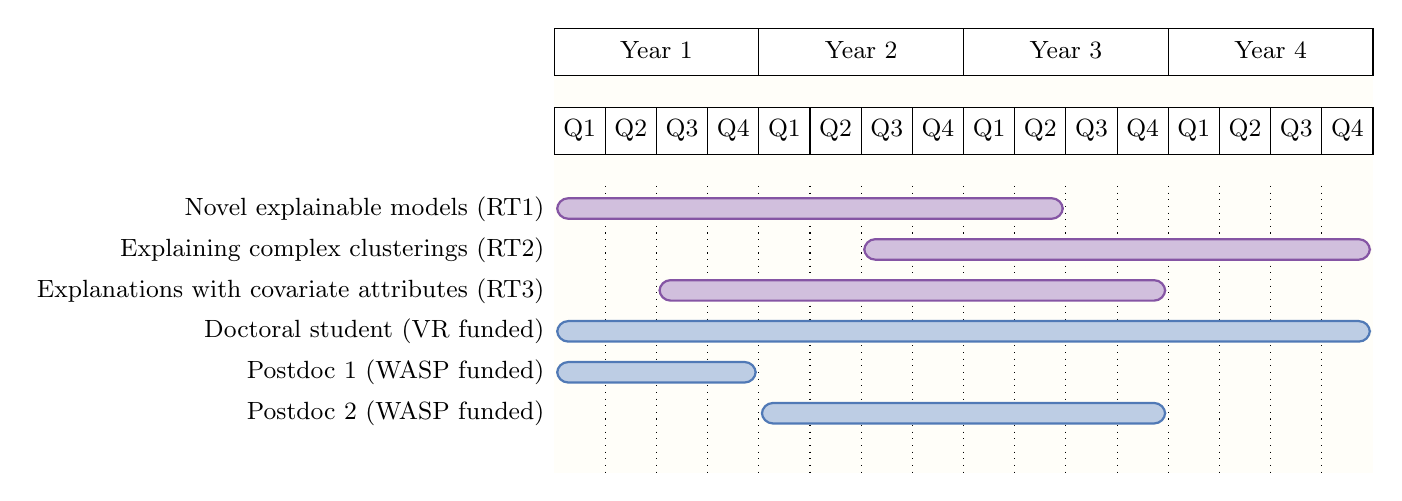
\begin{tikzpicture}
\ganttset{bar height=0.50}
\begin{ganttchart} [
	canvas/.style={fill=yafcolor6!03, very thick},
	x unit=.65cm,
	y unit chart = 0.52cm, 
	hgrid = false,
	vgrid = true, 
	bar right shift=-.06,
	bar left shift=.06,
	milestone/.style={draw=yafcolor3!90,fill=yafcolor3!60, thick}, 
	milestone height = 0.50
]{1}{16}
\gantttitle{\small Year 1}{4} 
\gantttitle{\small Year 2}{4} 
\gantttitle{\small Year 3}{4} 
\gantttitle{\small Year 4}{4} 
\\
% year 1
\gantttitle{\small Q1}{1}
\gantttitle{\small Q2}{1}
\gantttitle{\small Q3}{1}
\gantttitle{\small Q4}{1} 
% year 2
\gantttitle{\small Q1}{1}
\gantttitle{\small Q2}{1}
\gantttitle{\small Q3}{1}
\gantttitle{\small Q4}{1} 
% year 3
\gantttitle{\small Q1}{1}
\gantttitle{\small Q2}{1}
\gantttitle{\small Q3}{1}
\gantttitle{\small Q4}{1} 
% year 4
\gantttitle{\small Q1}{1}
\gantttitle{\small Q2}{1}
\gantttitle{\small Q3}{1}
\gantttitle{\small Q4}{1} 
\\
\ganttbar[bar/.style={rounded corners,inner sep=0pt,thick,draw=yafcolor1!80,fill=yafcolor1!30}]
{\small Novel explainable models (\rto)}{1}{10} \\
\ganttbar[bar/.style={rounded corners,inner sep=0pt,thick,draw=yafcolor1!80,fill=yafcolor1!30}]
{\small Explaining complex clusterings (\rtw)}{7}{16} \\
\ganttbar[bar/.style={rounded corners,inner sep=0pt,thick,draw=yafcolor1!80,fill=yafcolor1!30}]
{\small Explanations with covariate attributes (\rth)}{3}{12} \\

\ganttbar[bar/.style={rounded corners,inner sep=0pt,thick,draw=yafcolor5!80,fill=yafcolor5!30}]
{\small Doctoral student (VR funded)}{1}{16} \\
\ganttbar[bar/.style={rounded corners,inner sep=0pt,thick,draw=yafcolor5!80,fill=yafcolor5!30}]
{\small Postdoc 1 (WASP funded)}{1}{4} \\
\ganttbar[bar/.style={rounded corners,inner sep=0pt,thick,draw=yafcolor5!80,fill=yafcolor5!30}]
{\small Postdoc 2 (WASP funded)}{5}{12} \\
\end{ganttchart}
\end{tikzpicture}


% \begin{ganttchart}[
% 	vgrid,
% 	progress=today,
% 	progress label text=\relax,
% 	today=6
% ]{1}{12}
% \gantttitlecalendar{day} \\[grid]
% \ganttfoobar{Foobar 1}{1}{2} \\
% \ganttfoobar{Foobar 2}{3}{7} \\
% \ganttlinkedfoobar{Foobar 3}{9}{12}
% \end{ganttchart}}
\end{center}
\vspace{-6mm}
\caption{\label{figure:gantt}The time schedule of {\acronym}.}
\vspace{-2mm}
\end{figure}

The time schedule of \acronym is depicted in Figure~\ref{figure:gantt}. 
The diagram shows the duration of the research themes over the lifetime of the project
and the personnel working on the project.

The funding by the Swedish Research Council will be used to recruit 
one doctoral student who will work exclusively on this project, 
in addition to their teaching duties in KTH.
The doctoral student will be funded at 80\% level from this project, 
and the remaining 20\% will be provided from KTH for the student's teaching duties. 
At this level of research activity, the expected completion time of the doctoral student is 5 years. 
The fifth year, after the completion of the project, 
will be provided by KTH basic funding allocation to the PI, or other external funding source. 

The PI will allocate 12\% of his time on this project.
In addition, two postdoctoral researchers in the research team of the PI
will work on the project at 50\% of their time. 
The time of the postdocs will be funded by the WASP recruitment package of the PI, 
thus, increasing the added value of this project.
The first postdoctoral researcher is Sebastian Dalleiger, 
who is already a member of the research team, 
while the second postdoc will be recruited in the second year of the project.

In terms of the work allocation on the research themes, 
the PI will work on all research themes and will supervise the work of the other team members. 
The doctoral student will work on research themes \#1 and \#2, 
as those are the most closely related and there are many interesting research questions
and ample potential for new methods to develop that fulfill the requirements for a doctoral dissertation. 
The postdocs, together with the PI, will focus on carrying out research theme \#3,
while also helping to supervise the doctoral student on themes \#1 and \#2.

\spara{Research output.}
We will aim publishing our work at top-tier international venues, 
focus on quality rather than quantity.
% 
% in the areas of Knowledge Discovery, Machine Learning, and Artificial Intelligence.
% We will focus on the quality of publications rather than quantity.
Target journals 
% for disseminating our work 
are IEEE TKDE, PVLDB, ACM TKDD,  DMKD, etc. 
Target conferences are NeurIPS, ICML, ICLR, SIGMOD, SIGKDD, WebConf, WSDM, etc.

\spara{Materials.}
Our publications will be available via open access in {\small\url{arxiv.org}}. 
The software and the other outputs of the project 
will become freely available to the scientific community via {\small\url{github.com}}. % and archived in {\small\url{zenoodo.org}}.

\spara{Risks and mitigation.}
Devising efficient algorithms with provable quality guarantees is a challenging task
and the largest risk of the project. 
Achieving this objective, however, offers the largest potential for scientific impact.
%  in the computer science community. 
If we are not able to prove theoretical results, 
we will study problems with simplifying assumptions, and 
will focus on devising heuristic methods and providing thorough empirical validation.
Another risk is recruiting strong team members for the project. 
To mitigate this risk, we will leverage our international network
and the excellent reputation of the research group and research environment in Sweden. 
All the members of the project will be also affiliated with the WASP program, 
which will provide further incentive for recruitment and opportunities 
for network and collaborations during the project.


\subsection*{5.3~~~Project organization}

% \instructions{
% Clarify how you and any participating researchers will contribute to the implementation of the project. Explain in particular how the time allocated by you (that is, your activity level) as project leader is suitable for the task, including the relationship with your other research undertakings. Describe and explain the competences and roles of the participating researchers in the project, and also other key persons (including any doctoral students) who are important for the implementation of the project.
% }

The PI will devote 12\% of his time in the project. 
He will supervise the doctoral student and two postdocs, 
be responsible for scientific lead, 
and will allocate time to work on mathematical and algorithmic problems.
He will be responsible for ensuring flow of information and collaborations
with other groups in KTH and his international collaboration network, 
offering the possibility to the group to make research visits and internships.
The PI is currently managing an ERC Advanced Grant (2020 to 2026),
which employs 3 doctoral students and 3 postdocs, 
so the ERC project will be ending during the first year of this project. 
In addition, the PI is still utilizing resources from his WASP recruitment package, 
which are not tied to any specific research project, 
and as explained in the previous section part of those resources will be allocated to the {\acronym} project.

% The doctoral students and postdocs will work in pairs on the corresponding research theme.
For the work in research team, 
we will encourage an environment of openness and collaboration, 
while ensuring that each team member leads their own project.
%
During the hiring process we will support diversity and consider actions to achieve gender balance. 
Currently the PI supervises 6 doctoral students and the gender ratio is 3:3.


% \subsection*{Equipment {\color{orange}[$\approx$0.2 page]} {\color{teal}(Aris)}}

% \instructions{
% Describe the basic equipment you and your team have at your disposal for the project.
% }

\subsection*{6~~~Equipment and need for research infrastructure}

% \instructions{
% Specify the project’s need for international and national research infrastructure. If you choose to use other infrastructure than those supported by the Swedish Research Council External link.and that are thereby open to all, you must justify this (also applies to local research infrastructure).
% }

The project is mainly of theoretical nature and will not require extensive computing infrastructure. 
Commodity laptops will be provided to all team members. 
For implementing and evaluating our methods we will use the available 
KTH computing facilities
and the National Academic Infrastructure for Supercomputing in Sweden (NAISS).
The team has also access to the Berzelius supercomputer, 
available to WASP-affiliated faculty, 
which is among the world's 100 fastest AI supercomputers.

\subsection*{7~~~International and national collaboration}

% \instructions{
% Describe your own and the team’s collaboration with foreign and Swedish researchers and research teams. State whether you contribute to or refer to international collaboration in your research.
% }

The PI has an extensive international collaboration network. 
Recent and ongoing collaborations include
prof.\ De Bie in Ghent University, 
prof.\ Terzi in Boston University,
prof.\ Mannila in Aalto University, and 
Dr.\ Bonchi in Centai Labs.
In spring 2024 the PI will spend one month as a visiting professor 
in Sapienza University of Rome, hosted by prof.\ Leonardi.
In the near future the PI will apply for a sabbatical in Stanford University, 
planning to visit prof.\ Ugander. 
We will seek to strengthen and further expand this collaboration network.
We will encourage the research team to be actively involved in national and international collaborations
and make research visits and internships in other institutes.

\subsection*{8~~~Independent line of research}

% \instructions{
% If you are working or will be working in a larger group, please clarify how your project relates to the other projects in the group. If you are (continuing) working in the same team as your doctoral or postdoc supervisor, or if you are continuing a project that wholly or partly started during your doctoral or postdoc studies, you must also describe the relationship between your project and the research of your former supervisor.
% }

This is a new line of research in our group. 
We have recently worked on data clustering~\cite{spoerhase2023constant,thejaswi2021diversity}
and on explainable supervised-learning~\cite{ciaperoni2023concise,zhang2020diverse,zhang2023regularized}, 
but research in explainable unsupervised learning is novel.


{\small
\setlength{\bibsep}{0pt}
\bibliographystyle{abbrv}
\bibliography{references}
}

% \newpage
% \input{rebound}

\end{document}




